\chapter{Anwendung des Frameworks auf jadice flow}
\label{chap:anwendung}

In diesem Kapitel wird ein Architektur-Refactoring am Produkt \emph{jadice flow} geplant und in theoretischer Ebene durchgeführt.
Dazu werden \acrfull{mmf} und \acrfull{arh} benutzt, welche den Prozess sowie auch dieses Kapitel in drei Phasen unterteilen.
Eine genauere Beschreibung des Frameworks ist in \cref{sec:mmf} zu finden, sehr abstrahiert und vereinfacht bestehen die Phasen aus folgenden Aktivitäten:
\begin{itemize}
	\item In \cref{sec:durchführung-phase1} wird die Durchführung der ersten Phase in Form eines Architekturreviews mit den wichtigsten Stakeholdern beschreiben.
	\item Im Rahmen der zweiten Phase wird in \cref{sec:durchführung-phase2} nach adäquaten Migrationsstrategien gesucht.
	\item In \cref{sec:durchführung-phase3} wird in der dritten Phase nach profitablen Patterns und Best Practices gesucht.
\end{itemize}

\section{Phase 1 - Systemverständnis}
\label{sec:durchführung-phase1}

Das Ziel dieser Phase ist ein Verständnis des Systems aufzubauen.
Dieses Verständnis ist wichtig für spätere Entscheidungen.

\subsection{Qualitätsattribute}

Im ersten Schritt dieser ersten Phase werden die gewünschten \glspl{qa} des Systems gesammelt.
In dieser Phase wurde in einer Fokusgruppe ein Architekturreview nach \Citet{SVAHNBERG20071893} wie in \cref{sec:methodik-architekturreview} beschrieben durchgeführt.
Teil dieser Gruppe waren vier Softwareentwickler beziehungsweise -Architekten, der \acrlong{po} und ich selbst in der Rolle des Moderators.
Durch die ebenfalls in \cref{sec:methodik-architekturreview} beschriebenen Veränderungen an der Methodik von \Citet{SVAHNBERG20071893} wurde auch der geplante Zeitrahmen dieser Fokusgruppe auf lediglich 2 Stunden reduziert. Das liegt vor allem daran, dass die letzten Phasen nicht nötig waren, aber auch daran, dass alle Teilnehmer bereits vertraut mit dem Produkt und der Architektur und Funktionsweise des Systems waren.
Demnach konnte nach einer kurzen Einleitung in die verwendete Methodik sofort mit Schritt 2, dem Ordnen der \glspl{qa} nach Wichtigkeit gestartet werden.
Dafür wurde
% Dabei handelt es sich um eine Architekturbewertungsmethode, die auf Szenarien-basierten Methoden wie \gls{saam} (\Citet{saam}) und \gls{atam} (\Citet{kazman_2000}) aufbaut.
% Stakeholder definieren gemeinsam gewünschte Szenarien und ordnen diesen \glspl{qa} zu.
% Außerdem wird den verschiedenen Szenarien jeweils ein Grad der Schwierigkeit und ein Grad der Wichtigkeit zugewiesen.
% Die resultierenden Szenarien können in den \gls{arh} eingegeben werden.

Das Ergebnis dieser Fokusgruppe sind die Szenarien, in der \cref{tab:scenarios} zu sehen sind.

\begin{landscape}
	\begin{figure}
		\centering
		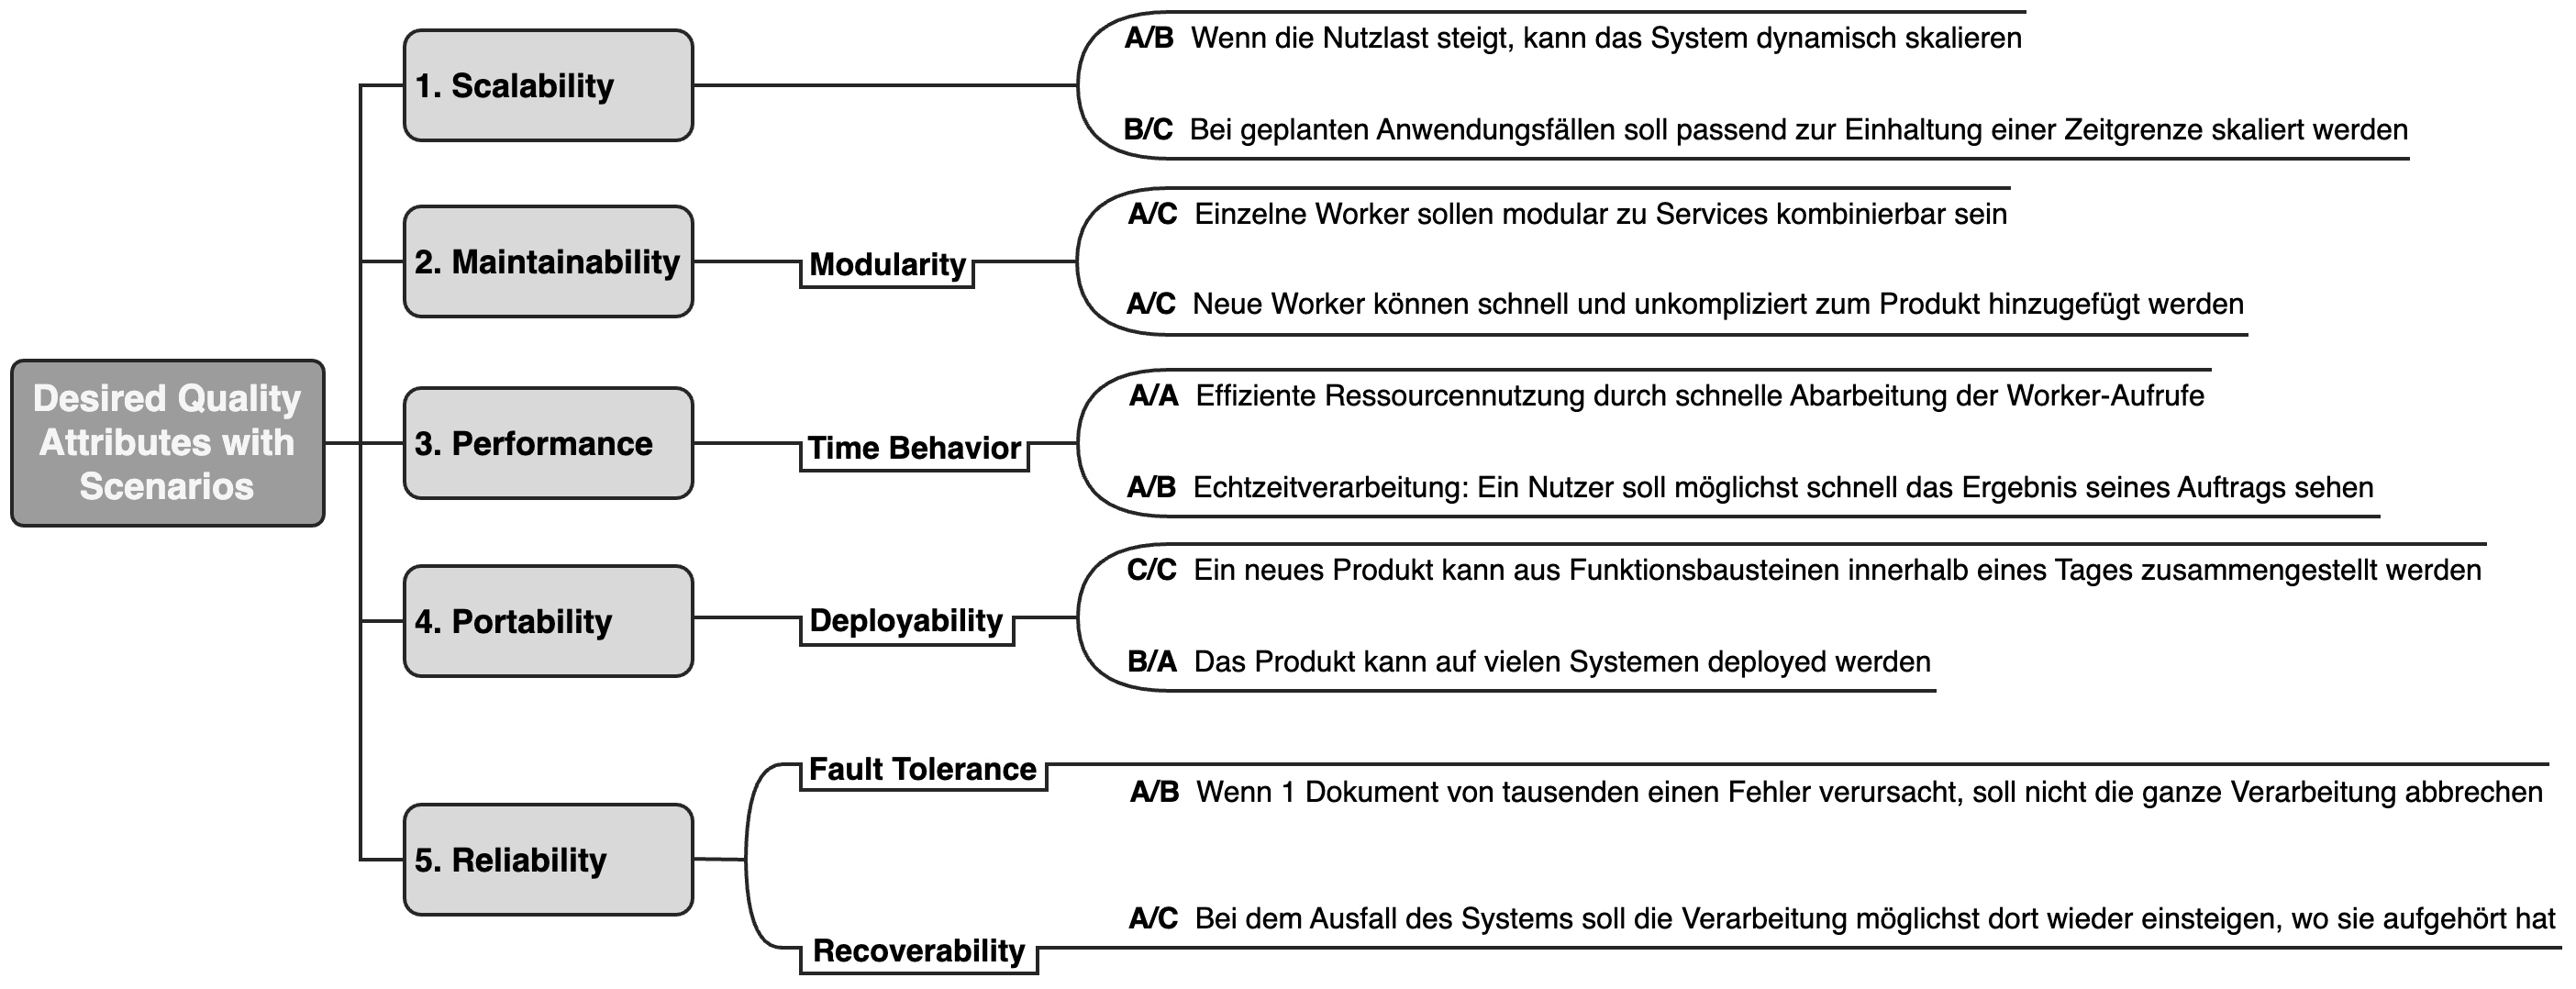
\includegraphics[width=1.5\textwidth]{scenarios.drawio}
		\caption[Utility Tree mit im Architekturreview ermittelten Qualitätsanforderungen und Szenarien]{
			Der Utility Tree mit Szenarien, die aus dem in Phase 1 durchgeführten Architekturreview resultieren.
			Von links nach rechts enthält der Baum folgende Elementarten: [1] Wurzel (ohne Bedeutung), [2] \gls{qa}, [3] Subattribut, [4] Beurteilung des Szenarios hinsichtlich Wichtigkeit und technischer Schwierigkeit, [5] Szenariobeschreibung.
		}
		\label{fig:scenarios}
	\end{figure}
\end{landscape}

Wie man in diesem Utility Tree sehen kann, sind die Szenarien nur mit jeweils einem \gls{qa} beziehungsweise Subattribut assoziiert.
Da realistischer Weise die meisten Szenarien allerdings mehrere \glspl{qa} beinhalten, wurden an einem zweiten Termin die Szenarien erneut betrachtet und diskutiert, welche weiteren \glspl{qa} sinnvoll hinzugefügt werden sollten.
Die resultierenden Assoziationen sind in der \cref{tab:scenarios} zu sehen.

\begin{table}[!h]
  \centering
  \begin{tabular}{ m{2,3cm} m{6cm} m{0.7cm} m{2,5cm} p{0.7cm} }
    \toprule
    \textbf{Name} & \textbf{Beschreibung} & \textbf{W/S} & \textbf{\glspl{qa}} & \textbf{MS} \\
    \midrule
    Dynamische Ska\-lier\-bar\-keit & Wenn die Nutzlast steigt, kann das Sys\-tem dynamisch skalieren & A/B & Scalability, Re\-source Uti\-li\-za\-tion, Adaptability, Execution Cost & \advantage \\ \hline
    Statische Ska\-lier\-bar\-keit & Bei geplanten Anwendungsfällen soll passend zur Einhaltung einer Zeitgrenze skaliert werden & B/C & Scalability, Resource Utilization, Time Behavior & \advantage \\  \hline
    Jobtemplates& Einzelne Worker sollen modular zu Services kombinierbar sein & A/C & Modularity, Reusability & - \\ \hline
    Neue Worker& Neue Worker können schnell und un\-kom\-pliziert zum Produkt hinzugefügt werden & A/C & Modularity, Reusability & \advantage  \\ \hline
    Schnelle Ab\-ar\-bei\-tung & Effiziente Ressourcennutzung durch schnelle Abarbeitung der Worker-Auf\-rufe  & A/A & Time Behavior, Resource Uti\-li\-za\-tion & \disadvantage \\ \hline
    \glqq Echtzeit\grqq{}-Verarbeitung & Ein Nutzer soll möglichst schnell das Ergebnis seines Auftrags sehen & A/B & Time Behavior & \disadvantage \\ \hline
    Einfaches De\-ploy\-ment & Ein neues Produkt kann aus Funk\-tions\-bausteinen innerhalb eines Tages zusammengestellt werden &C/C & Deployability, Modularity, Agility & \disadvantage \\ \hline
    Platform-unabhängigkeit& Das Produkt kann auf vielen Systemen deployed werden & B/A & Deployability, Installability & \advantage \\ \hline
    Fehlerto\-leranz Massen\-ver\-ar\-beitung & Wenn 1 Dokument von tausenden einen Fehler verursacht, soll nicht die ganze Verarbeitung abbrechen & A/B & Fault-Tolerance &\advantage \\ \hline
    Erholen nach Sys\-tem\-ausfall & Bei dem Ausfall des Systems soll die Verarbeitung möglichst dort wieder einsteigen, wo sie aufgehört hat & A/C & Recoverability & - \\
    \bottomrule
  \end{tabular}
  \caption[Im Architekturreview ermittelte Qualitätsanforderungen und Szenarien]{
    Szenarien, die aus dem in Phase 1 durchgeführten Architekturreview resultieren.
    \emph{W/S} gibt die Wichtigkeit/Schwierigkeit der Szenarien in drei Stufen an (A steht für sehr wichtig und sehr schwierig).
    \emph{\glspl{qa}} gibt die Assoziation der Szenarien zu bestimmten \acrfullpl{qa} an; zuerst genannte sind primäre \glspl{qa}, folgende sekundäre \glspl{qa}.
    \emph{MS} gibt die Einschätzung darüber an, ob das jeweilige Szenario von einer Microservices-Architektur profitiert.
  }
  \label{tab:scenarios}
\end{table}


Außerdem ist darin für jedes Szenario eine Einschätzung darüber enthalten, ob eine Microservices-Architektur für das spezifische Szenario von Vorteil ist (gegenüber einer monolithischen Architektur).
Da insgesamt in fünf Fällen eine Microservices-Architektur als profitabel und nur in drei Fällen als unvorteilhaft eingeschätzt wurde, kann die Entscheidung der Migration zu einer Microservices-Architektur durch diese Metrik bestärkt werden.
Außerdem ist anzumerken, dass die Szenarien in der Tabelle nach der Wichtigkeit der primären \glspl{qa} sortiert sind und die obersten zwei Szenarien der hauptsächliche Treiber für die Migration zu einer Microservices-Architektur waren.

\section{Phase 2 - Strategieplanung}
\label{sec:durchführung-phase2}

In dieser Phase werden die Ergebnisse der Phase 1 in Form von \glspl{qa} beziehungsweise Szenarien genutzt, um eine passende Migrationsstrategie zu finden.
Dazu wurden die in \cref{tab:scenarios} dargestellten Szenarien bereits in den \gls{arh} eingegeben.
Zusätzlich werden in dieser Phase Filterkriterien definiert.
Mit deren Hilfe wird dann schlussendlich eine Liste von Migrationsstrategien vorgeschlagen, welche folgend analysiert wird.

\subsection{Filterselektion}
Damit bei der Suche nach Migrationsmethoden möglichst gut zum Zielsystem und den Vorstellungen der Architekten passende Ergebnisse vorgeschlagen werden, bietet der \gls{arh} neben der Konfiguration der Szenarien noch eine weitere Art, die Ergebnisse zu filtern und ordnen: Die Filter, die in diesem Abschnitt konfiguriert werden.
Dabei kann für jede der Eigenschaften aus \cref{tab:phase2-filter} eine dieser drei Präferenzen angegeben werden:
\begin{itemize}
	\item \textbf{Include:} Methoden, die die jeweilige Eigenschaft haben, werden höher platziert.
	\item \textbf{Neutral:} Ob Methoden die jeweilige Eigenschaft haben, wirkt sich nicht auf ihre Platzierung aus.
	\item \textbf{Exclude:} Methoden, die die jeweilige Eigenschaft nicht haben, werden höher platziert.
\end{itemize}

\begin{table}
  \centering
  \begin{tabular}{m{2cm} m{2cm} m{9cm}}
    \toprule
    \textbf{Kategorie} & \textbf{Subkategorie} & \textbf{Eigenschaften} \\
    \midrule
    Quality Preferences & System Properties & Autonomy, Cohesion, Complexity, Coupling, Granularity, Isolation, Technology Heterogenity \\ \hline
    \multirow{4}{=}[-1cm]{Input Preferences} & Domain Artifacts &  Documentation, Human expertise, Ontology, Version Control System \\ \cline{2-3}
    & Runtime artifacts & Log traces, User-Application interactions \\ \cline{2-3}
    & Model artifacts & Activity diagram, Business process model, Class diagram, Custom model, Data flow diagram, Entity model, State machine diagram, Use case model \\ \cline{2-3}
    & Executables & API / Interface, Database file, Source code (Java), Source code (No specification), Source code (Python), Test cases \\ \hline
    \multirow{6}{=}[-1.9cm]{Process Preferences} & Directions & Bottom-up, Mixed, Top-down \\ \cline{2-3}
    & Levels of automation & Automatic, Manual, Semi-automatic \\ \cline{2-3}
    & Analysis types & Dynamic, Historic, Lexical, Static \\ \cline{2-3}
    & Techniques & Clustering, Custom heuristics, Data-flow driven, Domain-Driven Design, Execution-trace modeling, General guidelines, Genetic algorithm, Graph-based, Machine Learning, Multi-Tenancy, Performance modeling, Scenario analysis, Wrapping / Black Box \\ \cline{2-3}
    & Process Strategy & Continuous Evolution, Extension, Greenfield, Refactor, Rewrite / Rebuild, Strangler \\ \cline{2-3}
    & Atomar Unit & Business Capability, Class, Entity, Function, Functionality, Interface, Other \\ \hline
    Output Preferences & Representation & Guideline / Workflow, List of services, Source code, Splitting recommendations, Visualization \\ \hline
    \multirow{4}{=}[-1cm]{Usability Preferences} &Validation methods & Case study, Experiment, Industry, No validation \\ \cline{2-3}
    & Accuracy of \gls{sia} & High, Medium, Low, Not available \\ \cline{2-3}
    & Tool supports &  No tool support \\ \cline{2-3}
    & Tool types & Database, Decomposition, Dynamic Analysis, Java, Open Source, Other, Reverse Engineering, Static Analysis, Visualization \\
    \bottomrule
  \end{tabular}
  \caption[Mögliche Filter des \gls{arh} in Phase 2]{
    Mögliche Filter des \gls{arh} in Phase 2.
  }
  \label{tab:phase2-filter}
\end{table}


Die Qualität dieser Filterfunktion soll ebenfalls in dieser Arbeit evaluiert werden, weshalb folgend in \cref{sec:phase2-ergebnisdurchsicht} die Ergebnisse verschiedener Filter betrachtet und verglichen werden.
Dafür wurden die Filter für das Refactoring von \emph{jadice flow} wie folgt gewählt.
Das Vorgehen ist in \cref{feldnotiz:1} dokumentiert.

\subsection{Ergebnisdurchsicht}
\label{sec:phase2-ergebnisdurchsicht}

\section{Phase 3a - Architekturplanung}
\label{sec:durchführung-phase3}